\documentclass[12pt,letterpaper]{article}
\usepackage[margin=1in]{geometry}
\usepackage{fancyhdr}
\usepackage[utf8]{inputenc}
\usepackage{palatino}
\usepackage{microtype}
\usepackage{hyperref}
\usepackage{graphicx}
\usepackage{lastpage}
\usepackage[hang,small]{caption}
\usepackage{titlesec}
\usepackage{amsmath,amssymb}
\usepackage{multirow}

\renewcommand{\headrulewidth}{0pt}
\fancyfoot{}
\fancyfoot[C]{\sf Page \thepage\ of \pageref{LastPage}}
\pagestyle{fancy}

\titleformat{\section}{\bfseries\Large}{\arabic{\thesection}}{1em}{}
\titleformat{\subsection}{\bfseries\large}{\arabic{\thesection}.\arabic{\thesubsection}}{1em}{}
\titleformat{\subsubsection}{\itshape}{\arabic{\thesection}.\arabic{\thesubsection}.\arabic{\thesubsubsection}}{1em}{}

\setlength{\parindent}{0cm}
\setlength{\parskip}{0.8em}

\captionsetup[figure]{labelfont=it,font=it}
\captionsetup[table]{labelfont={it,sc},font={it,sc}}

\hypersetup{colorlinks,
    linkcolor = black,
    citecolor = black,
    urlcolor  = black}
\urlstyle{same}



\begin{document}

Soo-Hyun Yoo \\
ST314 \\
Data Analysis 1\\
October 8, 2014

\begin{enumerate}
	\item The following is a stem-and-leaf plot of the data:

		\begin{table}[!h]
			\centering
			\begin{tabular}{r|l}
				5 & 9 \\
				6 & 1 \\
				7 & 2 6 \\
				8 & 1 3 6 7 7 8 8 9 9 9 \\
				9 & 0 0 0 1 1 1 1 1 2 2 2 2 3 4 5 5 \\
			\end{tabular}
		\end{table}

		The scores are heavily skewed left with no outliers. Some statistics:

		\begin{table}[!h]
			\centering
			\begin{tabular}{|c|c|c|c|c|c|} \hline
				Mean & Median & StdDev & Lower 4th & Upper 4th & IQR \\ \hline
				86.833 & 90 & 8.891 & 86 & 92 & 6 \\ \hline
			\end{tabular}
		\end{table}

		The median makes more sense than the mean as an expression of
		the average. $\cfrac{13}{30}$ of the testers considered the
		wine truly exceptional. For a sample size of 500, however, it
		would be tedious to assemble a stem-and-leaf plot. A histogram
		would be a clearer display of the data.

	\item Plot and statistics:

		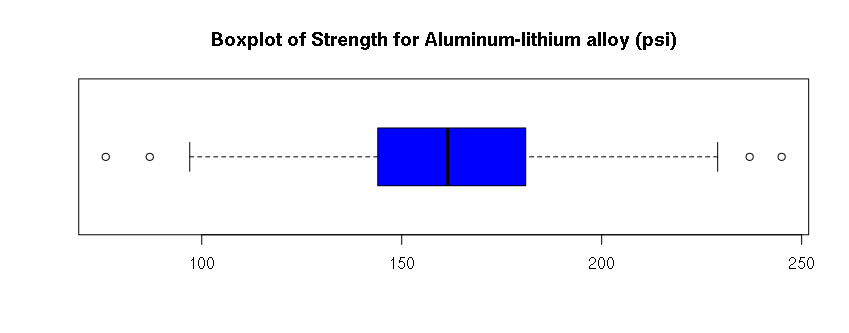
\includegraphics[width=0.9\textwidth]{p2.png}

		\begin{table}[!h]
			\centering
			\begin{tabular}{|c|c|c|c|c|c|} \hline
				Mean & Median & StdDev & Lower 4th & Upper 4th & IQR \\ \hline
				162.7 & 161.5 & 33.77 & 144.5 & 181.0 & 36.5 \\ \hline
			\end{tabular}
		\end{table}

		The compressive strengths of the specimens are balanced with a couple
		of outliers at both extremes. Because of this, either the mean or
		median would be a good estimate of the average value. The fairly narrow
		spread is good news for the users of the alloy because a given piece of
		stock will be more likely to possess the nominal compressive strength.

	\item Summary statistics:

		\begin{table}[!h]
			\centering
			\begin{tabular}{|c|c|c|c|c|c|c|} \hline
				& Mean & Median & StdDev & Lower 4th & Upper 4th & IQR \\ \hline\hline
				Unseeded & 164.60 & 44.20 & 278.45 & 24.82 & 159.20 & 134.38 \\ \hline
				Seeded   & 442.00 & 221.60 & 650.79 & 98.13 & 406.00 & 307.87 \\ \hline
			\end{tabular}
		\end{table}

		Both groups are heavily skewed right, with outliers at the upper end of
		the data. Consequently, the centers are located towards the lower ends
		of their respective groups. The spread is greater for the seeded group.

		The histograms make it easy to see the concentration of data points at
		the lower end of the unseeded group compared to the seeded group. The
		centers are more easily visible in the box plots, however. It is
		obvious that the seeded clouds promoted more rainfall than unseeded
		clouds, as the center and upper quartile values are pulled
		significantly to the right.
\end{enumerate}

\end{document}

